%\begin{frame} %-----------------------------%
%\frametitle{}
%  \begin{itemize} \item \vspace*{0.1cm} \end{itemize} 
%\end{frame}   %-----------------------------%


\section*{Introduction}  
%\subsection*{Introduction}

\begin{frame} %-----------------------------%
\frametitle{Motivation}
	\begin{itemize} 
	\item Application of Attitude Control and Estimation
		\begin{itemize} 
		\item \Emph{Space systems (spacecraft)} 
		\vspace*{0.1cm} 
		\item Atmospheric flight vehicles (quadrotors)
		\vspace*{0.1cm} 
		\item Underwater vehicles, ground vehicles, robotic systems 
		\end{itemize}  
	\vspace*{0.3cm}
\pause	
	\item Attitude Dynamics of A Rigid Body  
		\begin{itemize} 
		\item Attitude: orientation of a body-fixed frame with respect to a reference frame.
		\vspace*{0.1cm} 
		\item Special Orthogonal Group:
	    	\begin{align*} %SO(3)%
	       	\SO = \{ R\in\Re^{3\times 3}\,|\, R^TR=I,~\mathrm{det}[R]=1\}
	       	\end{align*}		
		\end{itemize} 
%	\vspace*{0.3cm}
	\end{itemize} 
        	\begin{figure} %figure%
            \centerline{
            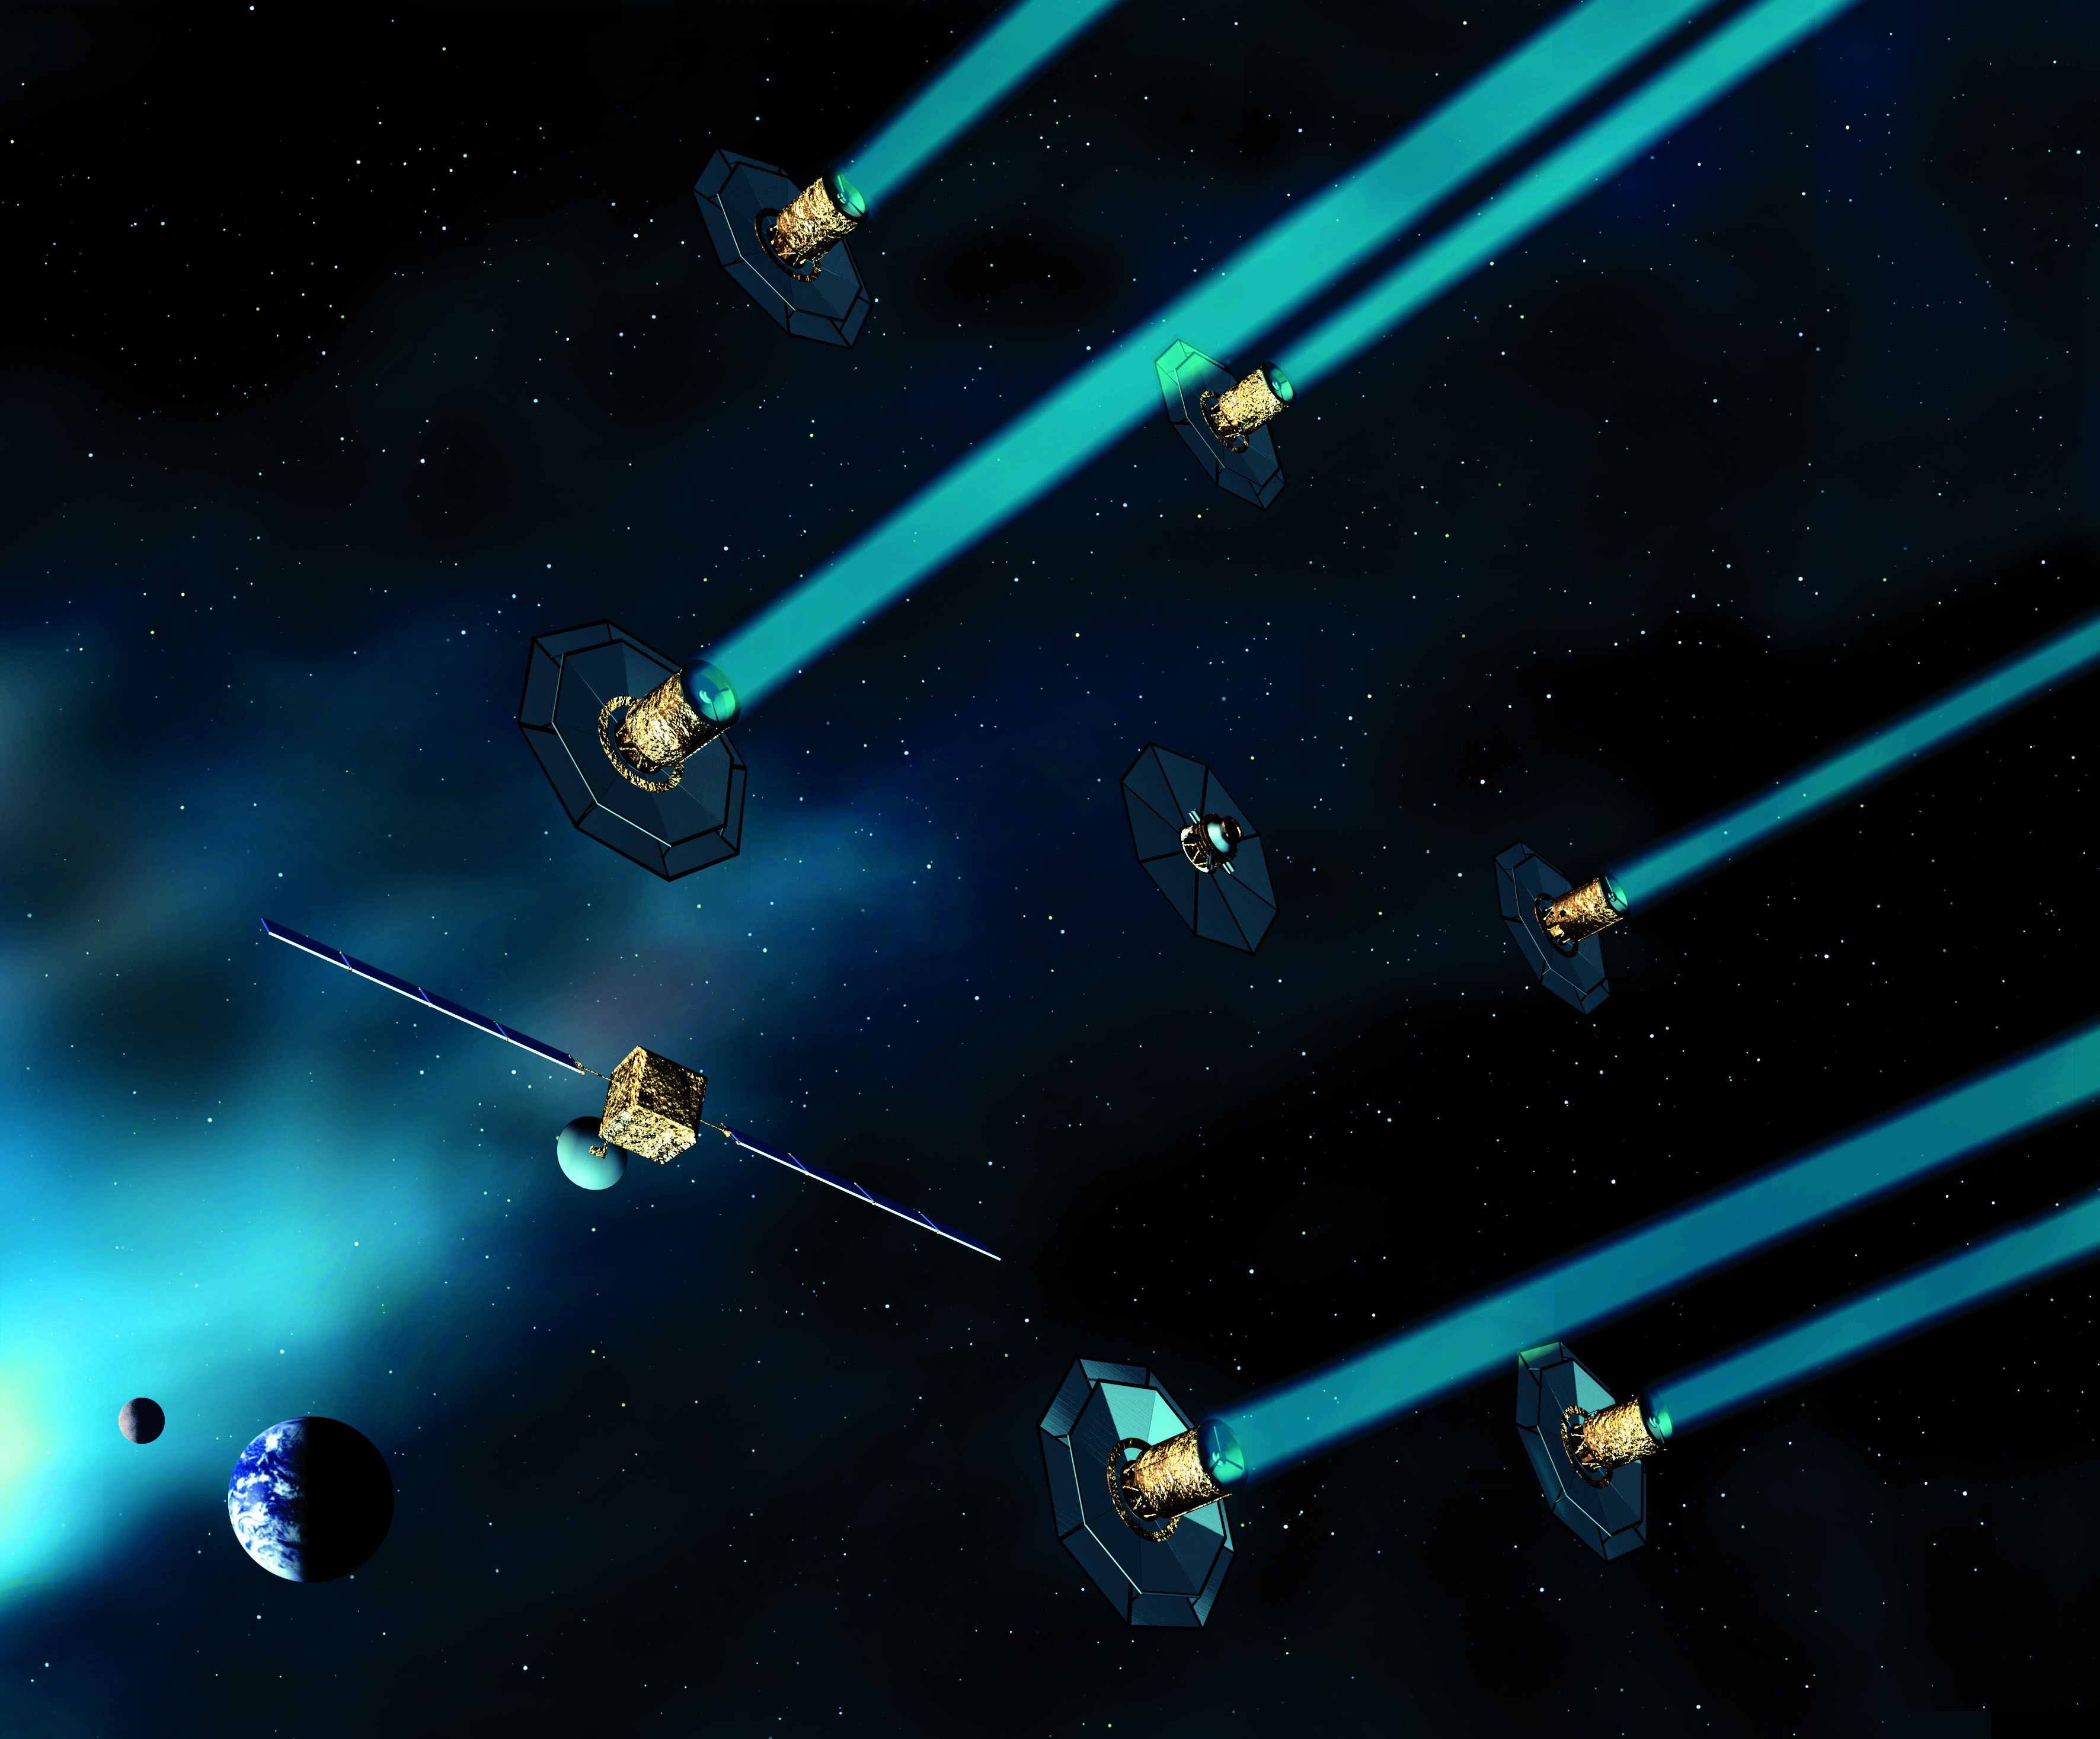
\includegraphics[width=2.4cm]{Mot_darwin1.jpg}\hspace*{0.3cm}
            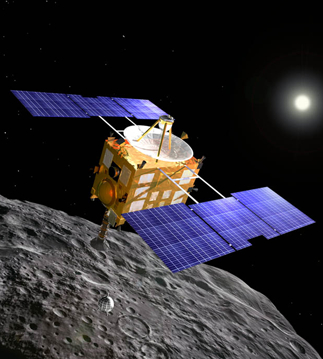
\includegraphics[width=1.81cm]{sat.jpg} \hspace*{0.3cm}
            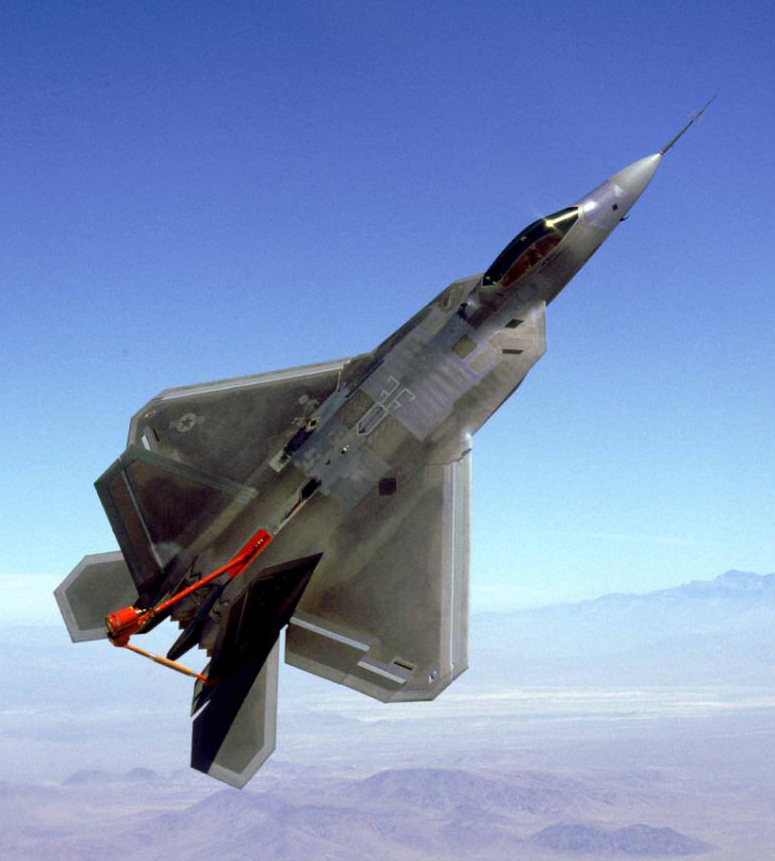
\includegraphics[width=1.8cm]{f22.jpg} \hspace*{0.3cm}
            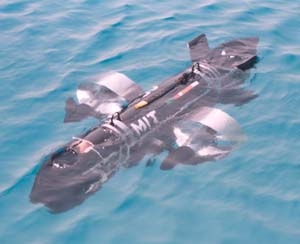
\includegraphics[width=2.49cm]{orca2b.jpg} 
            }
          	\end{figure}	
\end{frame}   %-----------------------------%



\begin{frame} %-----------------------------%
\frametitle{Geometric Control and Estimation}
\begin{itemize} 
\item Geometric Control and Estimation on Nonlinear Manifold 
	\begin{itemize} 
	\item Questions of \Emph{global nature} require global analysis for satisfactory solutions.
	\vspace*{0.1cm} 	
	\item Control and estimation systems are designed from the perspective of \Emph{differential geometry}.
%	\vspace*{0.1cm} 
%	\item ``Coordinate-invariant'' and ``intrinsic formulations''.
	\end{itemize} 
	\vspace*{0.3cm}
%\pause	
\item Geometric Control and Estimation on $\SO$	
	\begin{itemize} 
	\item \tc{purple}{No singularities} in representing large angle rotational maneuvers.
	\vspace*{0.1cm} 
	\item \tc{purple}{No ambiguities} and unwinding associated with quaternions.
	\vspace*{0.1cm} 
	\item Remarkably \tc{purple}{compact form} of equations of motion for complex aerospace systems.
	\end{itemize} 	
\end{itemize} 
\end{frame}   %-----------------------------%

\begin{frame} %-----------------------------%
\frametitle{Topological Obstruction}
\begin{itemize} 
\item Topological Obstruction of $\SO$
	\begin{itemize} 
	\item Global asymptotic stability: \\ Lyapunov stability + \Emph{global attractivity}. 	
	\vspace*{0.05cm} 
	\item \tc{purple}{No \textit{continuous} controller} can globally asymptotically stabilize an equilibrium of an attitude control system	[Bhat,~2000].
	\end{itemize} 
	\vspace*{0.2cm}	
\item Continuous Attitude Control Law
	\begin{itemize}
	\item \textit{Almost} global asymptotic stability: the region of attraction excludes only a set of zero measure. 
	\vspace*{0.05cm} 
	\item \Emph{Convergence rate is slow} when the initial state is closed to undesired equilibria.
	\end{itemize} 	
\pause	
	\vspace*{0.2cm}	
	\item Literature
		\begin{itemize} 
		\item Attitude observer/estimator on $\SO$: [Mahony,~2008], [Vasconcelos,~2009], [Sanyal,~2012].
		\vspace*{0.05cm} 
		\item Hybrid attitude control system: [Mayhew,~2013], [Lee,~2013].
		\end{itemize}
	
\end{itemize}	
\end{frame}   %-----------------------------%


%\begin{frame} %-----------------------------%
%\frametitle{}
%\begin{itemize} \item \vspace*{0.1cm} \end{itemize} 
%\end{frame}   %-----------------------------%


